\section{AS-IS}\label{sec:asis}

\subsection{Models}
\begin{figure}[htbp]
    \centering
        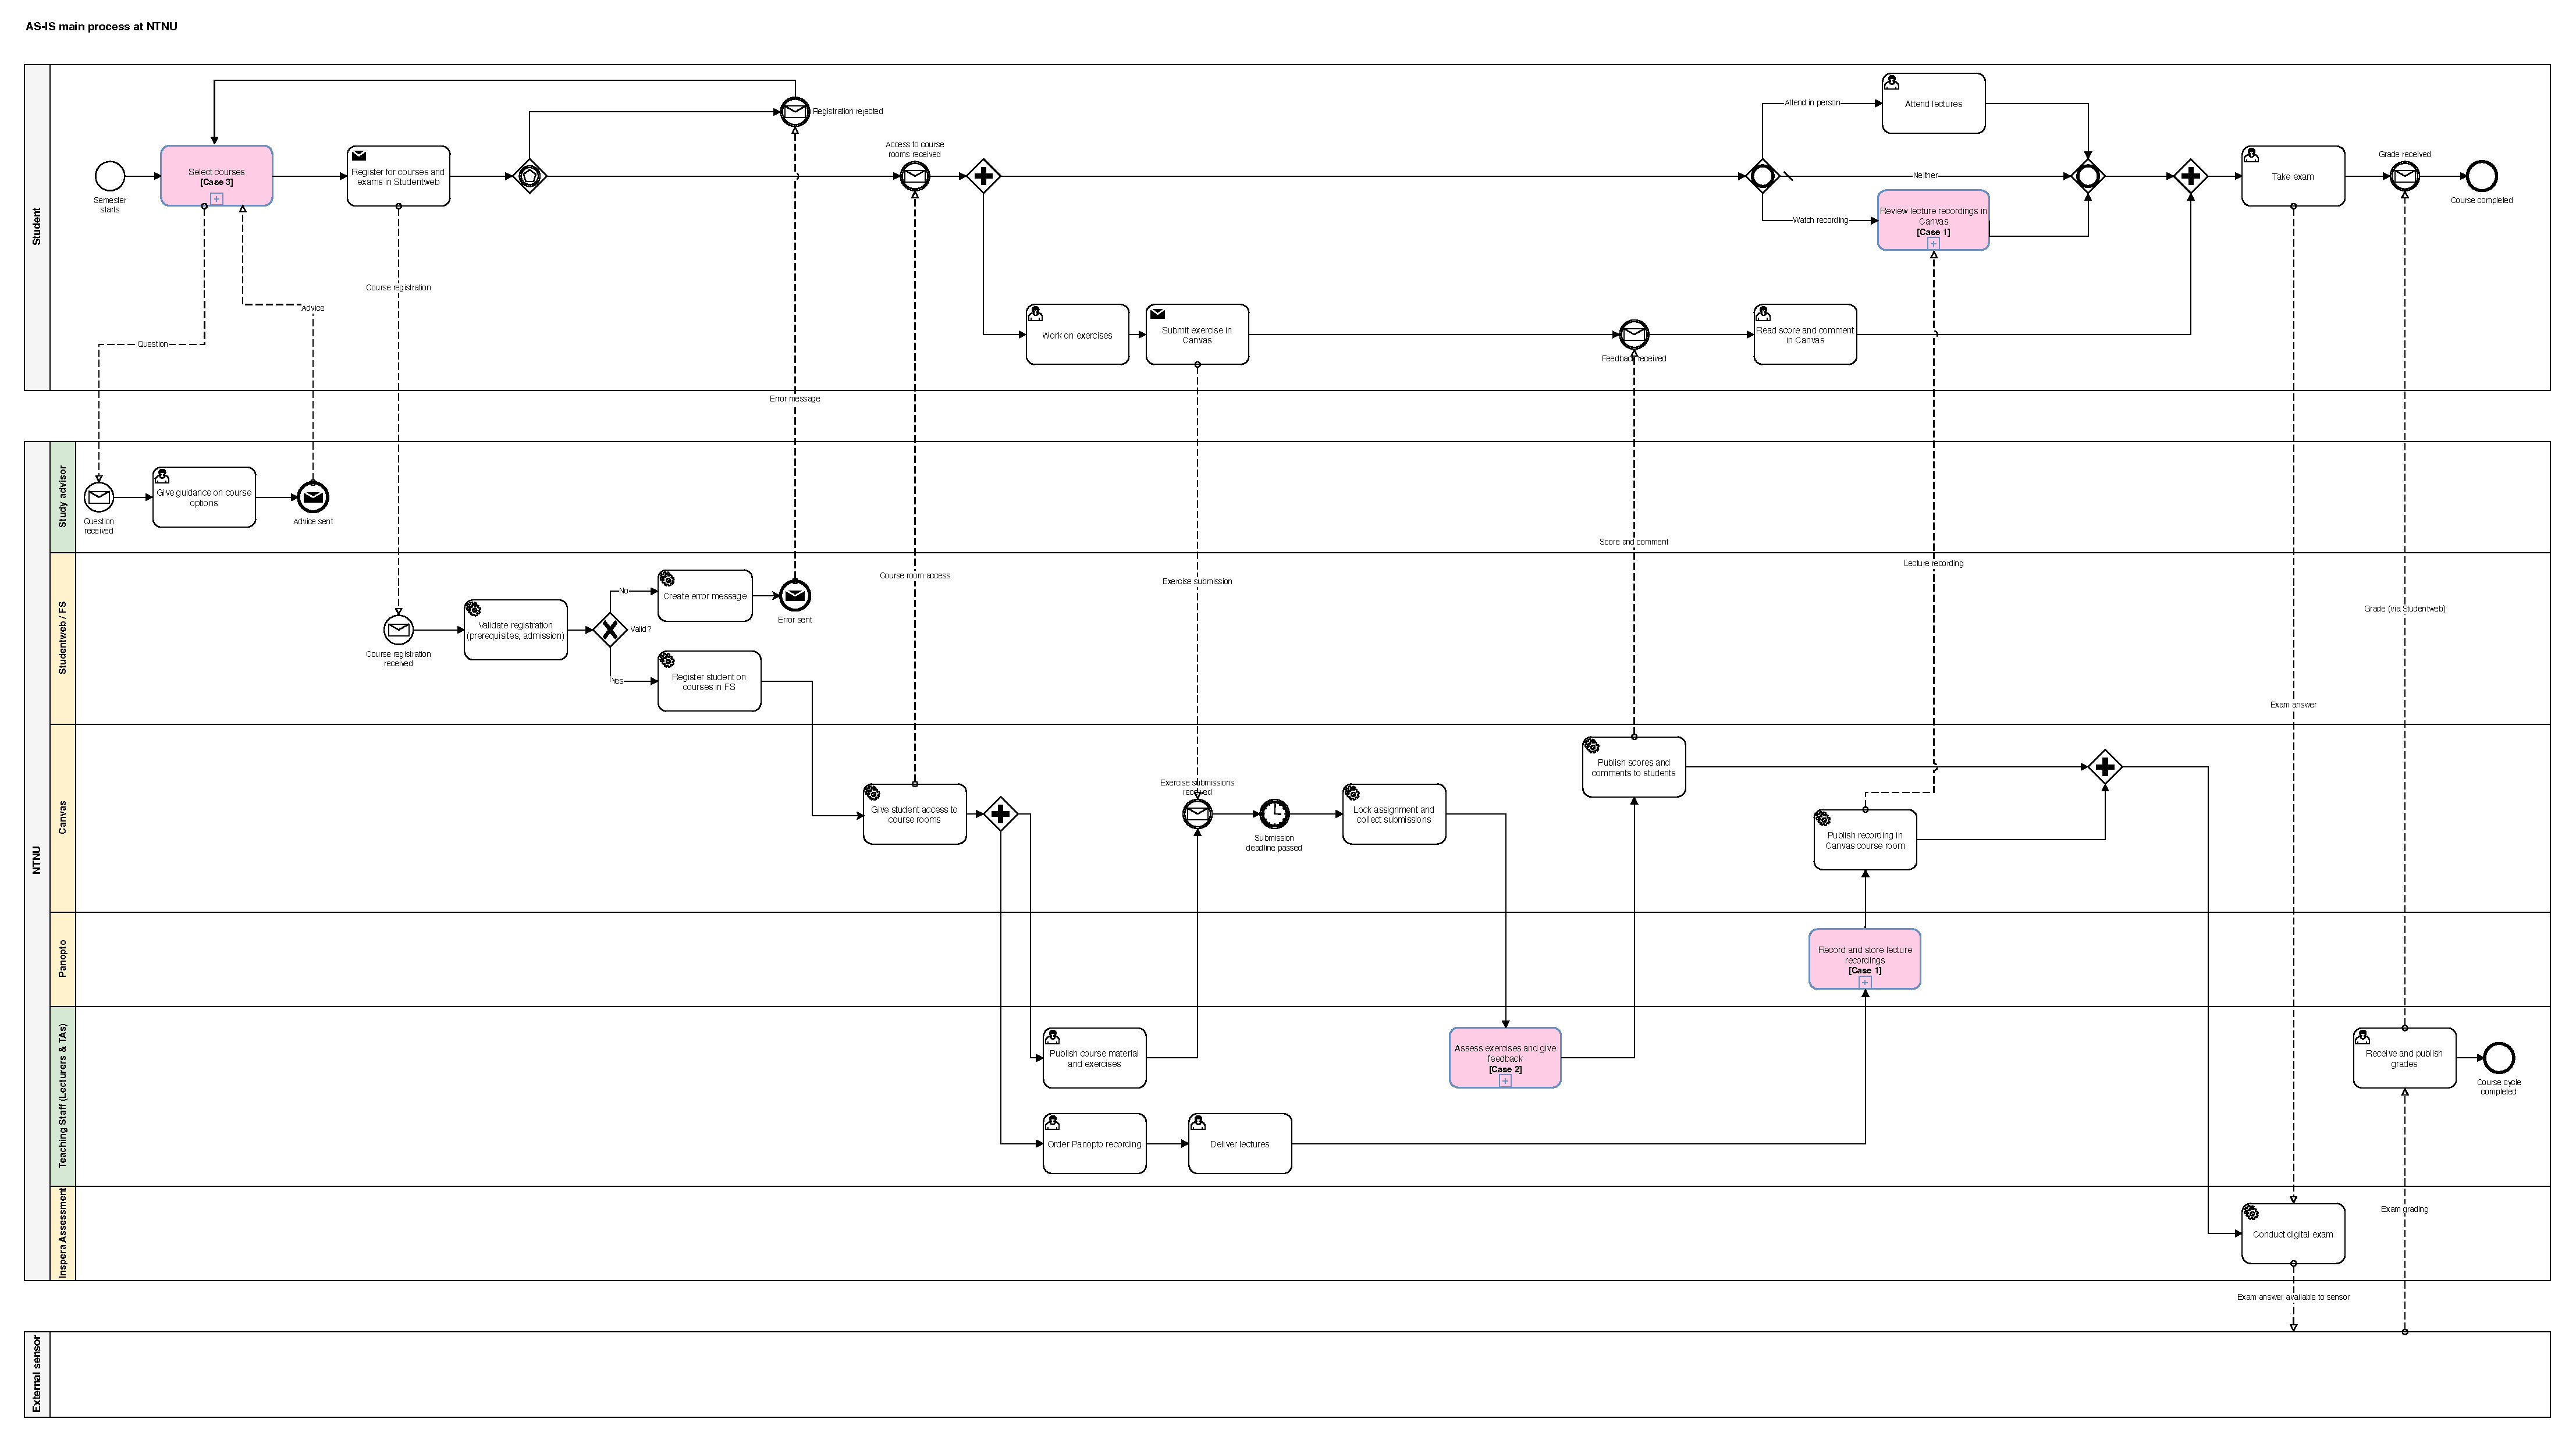
\includegraphics[width=\textwidth]{Images/main_as-is.drawio.pdf}
    \caption{AS-IS main process at NTNU}
    \label{fig:main_as-is}
\end{figure}

Figure~\ref{fig:main_as-is} presents a high-level BPMN model of the current (AS-IS) learning process at NTNU. The model consists of three pools: \textit{Student}, \textit{NTNU} and \textit{External sensor}. The NTNU pool is divided into lanes representing the actors and systems involved in the process: Study advisor, Studentweb/FS, Canvas, Panopto, Teaching Staff (lecturers and teaching assistants) and Inspera Assessment. Human actors are shown in green lanes and information systems in yellow lanes. The external sensor is modelled as a black-box pool. Collapsed sub-processes that are elaborated in the case models are marked pink.

\textbf{Course selection and registration:} The process starts at the beginning of the semester, when the student selects courses. This is modelled as the collapsed sub-process \textit{Select courses} (Case 3) in the Student pool. If the student needs advice, a question is sent to the Study advisor lane, where the study advisor gives guidance on the course options and sends the advice back to the student. When the courses have been selected, the student registers for courses and exams in Studentweb. The registration is received in the Studentweb/FS lane, where it is validated against the prerequisites and admission rules of each course. If the registration is valid, the student is registered on the courses in FS, and Canvas then gives the student access to the corresponding course rooms. If not, an error message is created and sent back to the student. On the student side, an event-based gateway waits for one of these two outcomes. If the registration is rejected, the student returns to course selection. If access to the course rooms is received, the learning activities of the semester begin.

\textbf{The learning phase:} The learning phase is modelled as two parallel tracks, one for lectures and one for exercises, both on the student side and on the NTNU side. In the lecture track, the teaching staff order a Panopto recording and deliver the lectures. The lectures are recorded and stored by Panopto in the collapsed sub-process \textit{Record and store lecture recordings} (Case 1), and Canvas then publishes the recording in the course room. On the student side, an inclusive gateway shows that the student may attend the lecture in person, watch the recording, or do both. The student's review of the recording is modelled as the collapsed sub-process \textit{Review lecture recordings in Canvas} (Case 1). Since lectures may not be mandatory, the gateway also has a default flow, \textit{Neither}, so that the student can skip the lecture track entirely.

In the exercise track, the teaching staff publish course material and exercises. The student works on the exercises and submits them in Canvas. When the submission deadline has passed, Canvas locks the assignment and collects the submissions. The teaching staff then assess the submissions in the collapsed sub-process \textit{Assess exercises and give feedback} (Case 2), before Canvas publishes the scores and comments to the students. The student receives the feedback and reads the score and comment in Canvas. Unlike the lectures, the exercises are mandatory and must be approved before the student can take the exam. This is why the two tracks are joined by a parallel gateway before the exam: the lecture track can be completed without any activity, while the exercise track must be completed in full. 

\textbf{Exam and grading:} When both tracks are completed, the student takes a digital exam in Inspera Assessment. On the NTNU side, a parallel gateway in the Canvas lane ensures that both the publishing of recordings and the publishing of feedback are completed before the exam is conducted. The exam answers are made available to the external sensor, who grades the exam and returns the result to NTNU. The teaching staff receive and publish the grades, and the student is notified of the final grade through Studentweb, which concludes the process.

The model is purposely kept at a high level of abstraction. Through our analysis of the current process, we have identified three parts of it where the current system support is insufficient, and where GenAI could make a clear improvement. These three cases are the focus areas of this project, and are modelled as collapsed sub-processes in the main model: \textit{Select courses} (Case 3), \textit{Record and store lecture recordings} and \textit{Review lecture recordings in Canvas} (Case 1), and \textit{Assess exercises and give feedback} (Case 2). Other activities are shown directly in the main model to provide context for the overall process. Each sub-process is elaborated in more detail in Section~\ref{subsec: Cases}.

\subsection{Cases}
\label{subsec: Cases}
\subsubsection{Case 1 - Lecture content is not searchable or reusable}
\textbf{Perceived problem:} Lecture recordings at NTNU (delivered via Panopto/Canvas) are stored as raw video with no transcription, summarization, or indexing. Students who want to review a specific concept must scrub through full recordings rather than search for it, and there is no automatically generated study material (summaries, key-point extraction, quiz questions) derived from lecture content. This underuses the opportunity for GenAI-based transcription and summarization, and creates inefficiency in how students prepare for exercises and exams.

% \textbf{Knut brukertester en forelesning}
% \begin{enumerate}
%     \item Knut går til canvas.ntnu.no
%     \item går inn på emnet tdt4175
%     \item trykker på panopto i menyen
%     \item kan der trykke på subsribe til emnet
%     \item åpner ønsket forelesning 
%     \item blir tatt til video view på panopto. 
%     \item Ser på video, får muligheten til å få oversikt over Contents
%     \item i Contents ser han at det er kapitler men satt til tittelen på hver slide (og ikke navnet på temaet/kapittelet). Så kan trykke seg frem og tilbake for å prøve å treffe det ønskede temaet
%     \item kan ta notater
%     \item det er ikke teksting/transkribering 
%     \item ikke delt opp i overordnet kapitler 
%     \item ikke gitt oppsummering 
%     \item Knut tar egne notater, bruker 3 timer på én forelesning som varer i 90 min.
%     \item Knut legger inn offentlige kommentater 
% \end{enumerate}

\begin{figure}[H]
    \centering
    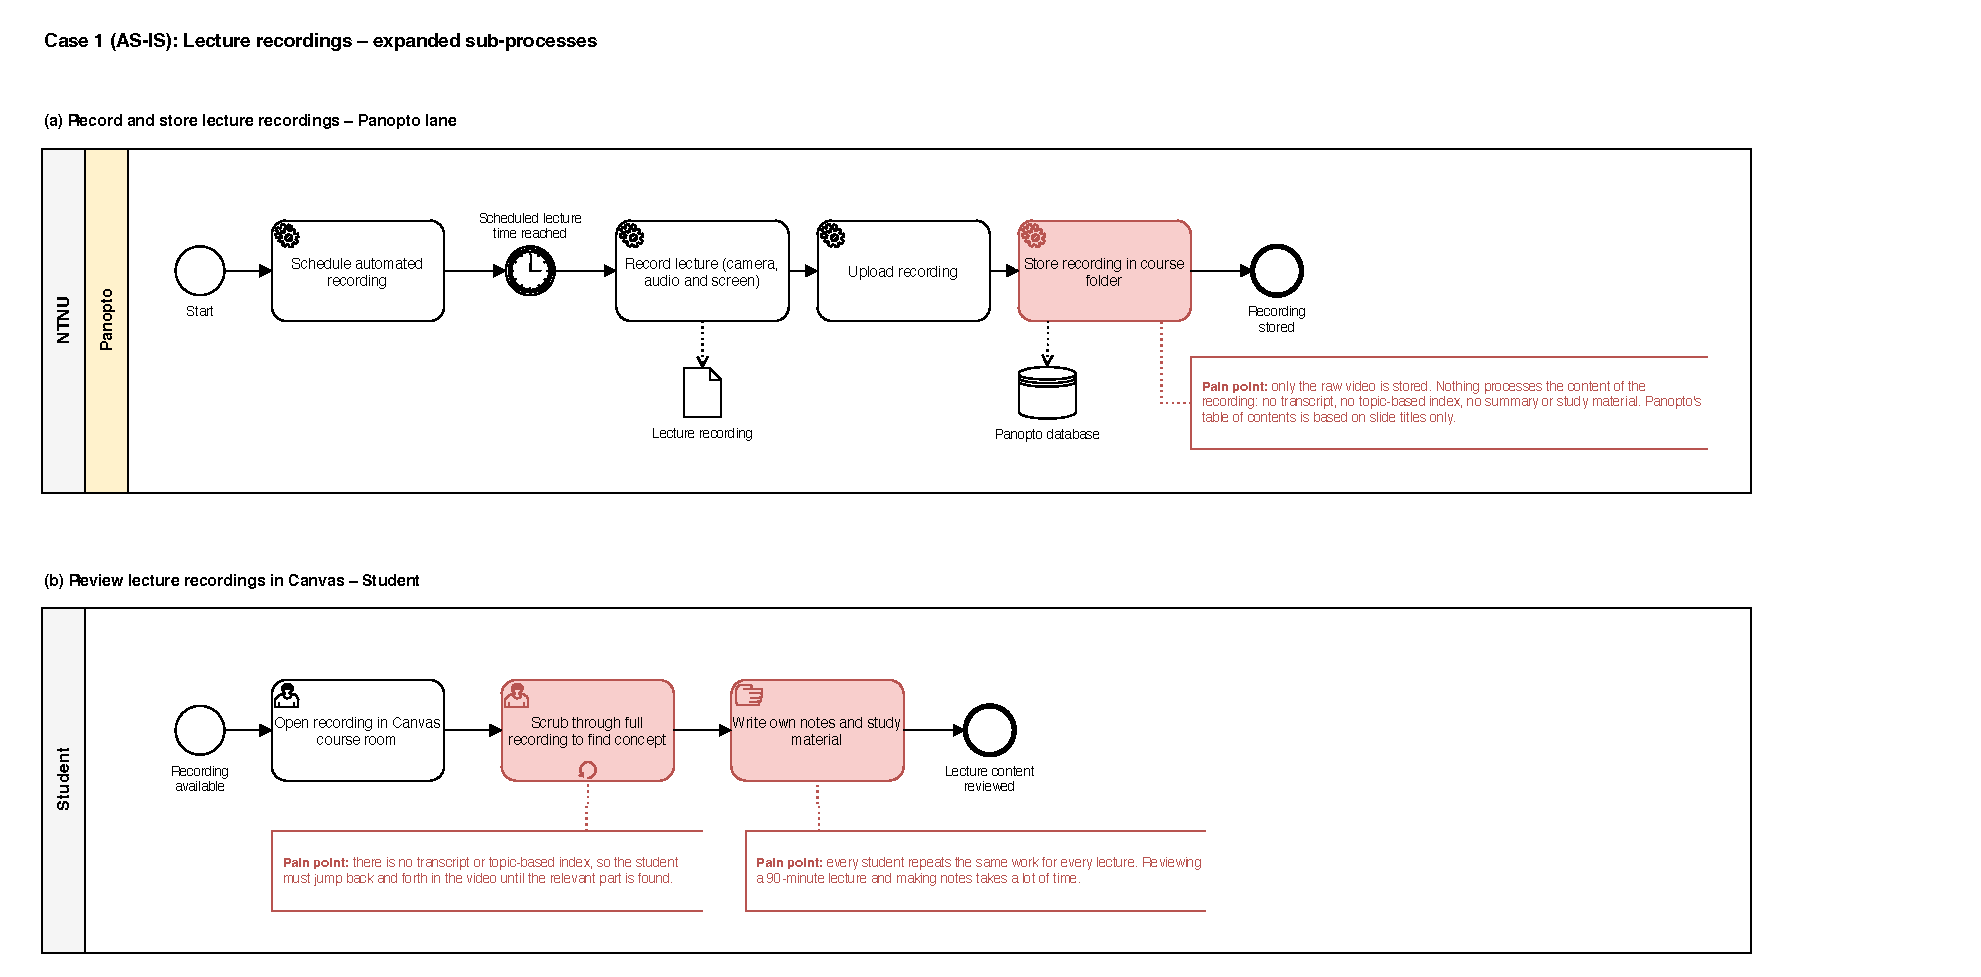
\includegraphics[width=\textwidth]{Images/case1/case1_as-is.drawio.pdf}
    \caption{Case 1 AS-IS BPMN models: (a) Record and store lecture recordings, (b) Review lecture recordings in Canvas}
    \label{fig:case1}
\end{figure}

\textbf{Model description:} Figure~\ref{fig:case1} expands the two collapsed subprocesses related to lecture recordings in the main model (Figure~\ref{fig:main_as-is}): (a) \textit{Record and store lecture recordings}, placed in the Panopto lane, and (b) \textit{Review lecture recordings in Canvas}, placed in the Student pool. Identified pain points are marked as red annotations in the model, and the activities they concern are marked red.

Subprocess (a) starts after the lecturer has ordered a Panopto recording in the main model. Panopto first schedules an automated recording, and the process then waits at the timer event \textit{Scheduled lecture time reached}. When the lecture starts, Panopto records camera, audio and screen. The output is the data object \textit{Lecture recording}. The recording is then uploaded and stored in the course folder in the \textit{Panopto database}, and the subprocess ends with \textit{Recording stored}. Back in the main model, Canvas makes the recording available in the course room.

Subprocess (b) starts when the recording is available in Canvas. The student opens the recording in the Canvas course room. The next activity, \textit{Scrub through full recording to find concept}, is modelled as a looping user task. Since the recording has no transcript or topic-based index, the student has to jump back and forth in the video until the relevant part is found. Finally, the student writes their own notes and study material. The subprocess ends with \textit{Lecture content reviewed}.

The model highlights three pain points. First, Panopto only stores the raw video. No activity processes the content of the recording, so there is no transcript, topic-based index, summary or study material. Panopto does generate a table of contents, but it is based on slide titles rather than topics. Second, because of this, the student must search for concepts by scrubbing through the video. Third, every student repeats the same work of reviewing the lecture and making notes, for every lecture. 
The recording process itself is efficient and fully automated, but the work of making the content usable is pushed onto each individual student. These pain points are the main targets for the TO-BE solution presented in Section~\ref{sec:4}.



\subsubsection{Case 2 - Feedback on exercises and assignments is minimal
}\textbf{Perceived problem}: Feedback on student exercises and assignments (via Canvas/Inspera)
is often limited to a numeric grade or a short generic comment, due to TA workload. Students receive
little actionable guidance on how to improve their writing, reasoning, or technical solutions,
which works against assisting the development of
students' writing skills and critical thinking/reflecting skills. There is no systematic
mechanism for scaling detailed, individualized feedback across large course cohorts.

\begin{figure}[h]
    \centering
    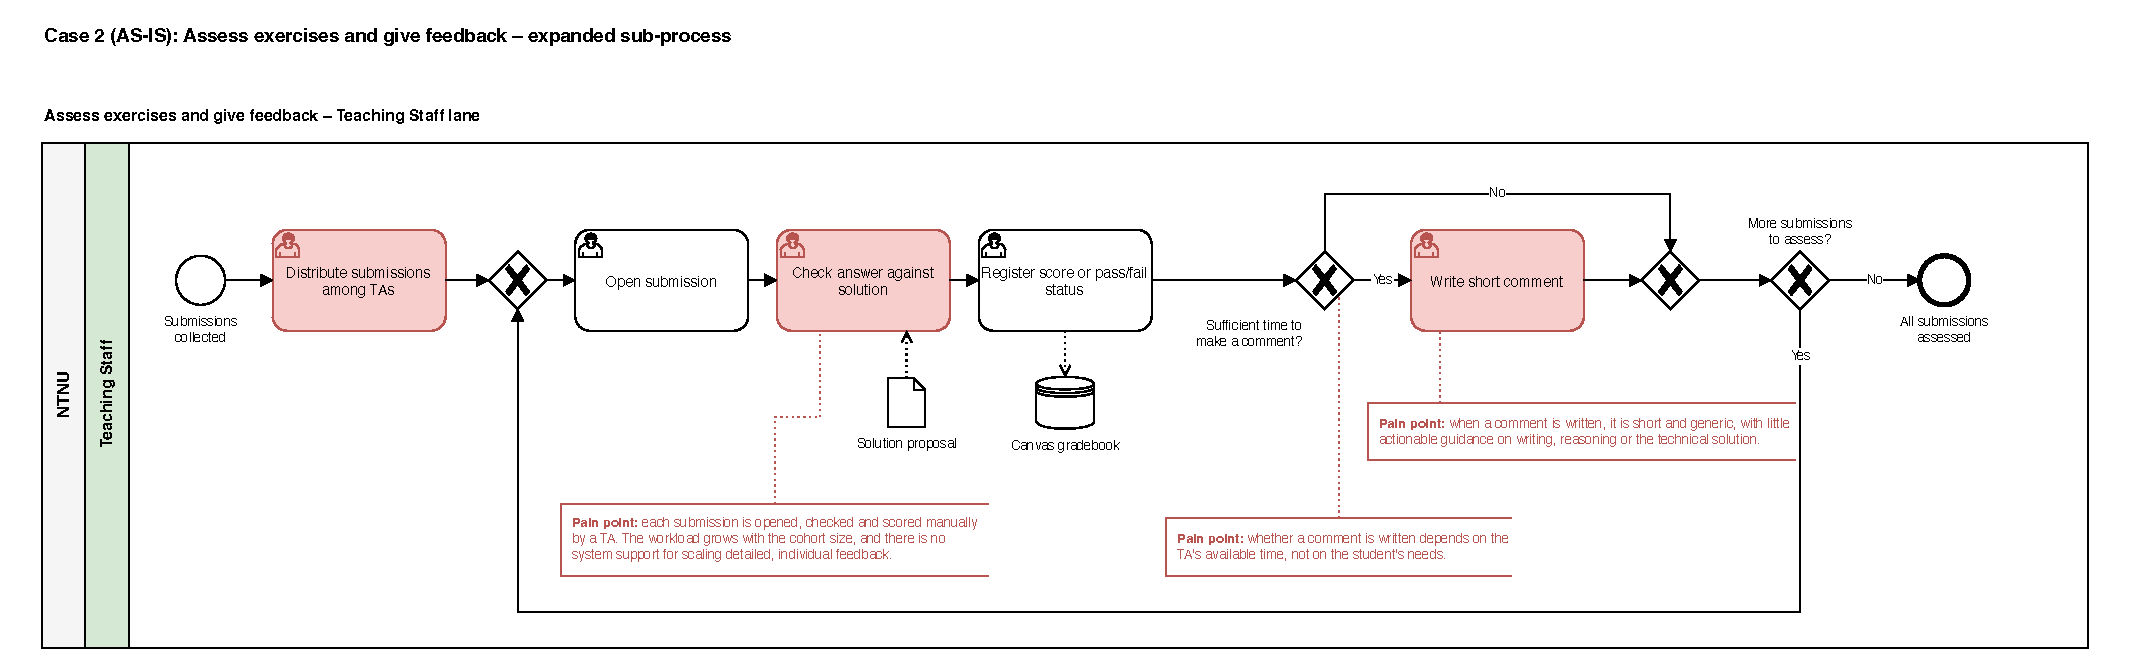
\includegraphics[width=\textwidth]{Images/case2/case2_as-is.drawio.pdf}
    \caption{Case 2 AS-IS BPMN model}
    \label{fig:case2}
\end{figure}

\textbf{Model description:} Figure~\ref{fig:case2} expands the collapsed subprocess \textit{Assess exercises and give feedback} in the Teaching Staff lane from the main model (Figure~\ref{fig:main_as-is}). Canvas receives the exercise submissions, and when the submission deadline has passed, it locks the assignment and collects the submissions. This starts the subprocess. Identified pain points are marked as red annotations in the model, and the activities they concern are marked red.

The subprocess starts when the submissions have been collected, and the teaching staff distribute them among the teaching assistants (TAs). The assessment is modelled as a loop that is repeated for each submission. The TA opens a submission and checks the answer against the solution proposal, which already exists and is shown as a data object in the model. The TA then registers a score or pass/fail status, which is stored in the Canvas gradebook. Next, an exclusive gateway represents the decision of whether there is sufficient time to make a comment. If so, the TA writes a short comment. If not, the comment is skipped, and the two paths merge again. A second exclusive gateway checks whether there are more submissions to assess. If there are, the flow returns to the start of the loop and the next submission is opened. When all submissions have been assessed, the subprocess ends with \textit{All submissions assessed}.

Back in the main model (Figure~\ref{fig:main_as-is}), Canvas publishes the scores and comments to the students, which sends the feedback to the student. In the Student pool, the student receives the feedback and reads the score and comment in Canvas before the exercise track continues towards the exam.

The model highlights three pain points. First, each submission is opened, checked and scored manually by a TA. The workload therefore grows with the size of the cohort, and there is no system support for scaling detailed, individual feedback. Second, whether a written comment is given depends on the time available to the TA, not on the needs of the student, so many students receive only a score. Third, when a comment is written, it is often short and generic, with little actionable guidance on writing, reasoning or the technical solution. The problem is therefore not that the TAs put too little effort into the feedback, but that the number of submissions leaves little time for each student. Students who want more detailed feedback must contact the teaching staff on their own initiative. These pain points are the main targets for the TO-BE solution presented in Section~4.2.


\subsubsection{Case 3 - Course selection and study plan personalization in Studentweb is static}
\label{sec:case3-asis}
\textbf{Perceived problem}: Studentweb lets students register for courses within a fixed program
structure, but offers no personalization based on individual interests, career goals, or prior
performance. Students choosing electives or specialization tracks must research options
manually across course catalogs and Innsida, with no system-supported recommendation of
which courses fit their profile or how to structure their remaining study plan. Many studyprogrammes at NTNU let students choose several electives courses, which gives them opportunity to shape their education towards the field they want to work in. Without guidance, however, it's difficult to know which courses fit a particular interest. As a result, students may choose courses that are not relevant to their goals, or miss courses they would have found more interesting. As a result, students face a static list of options with no guidance layered on top, instead of an adaptive selection process that supports personalized learning paths.


\begin{figure}[H]
    \centering
    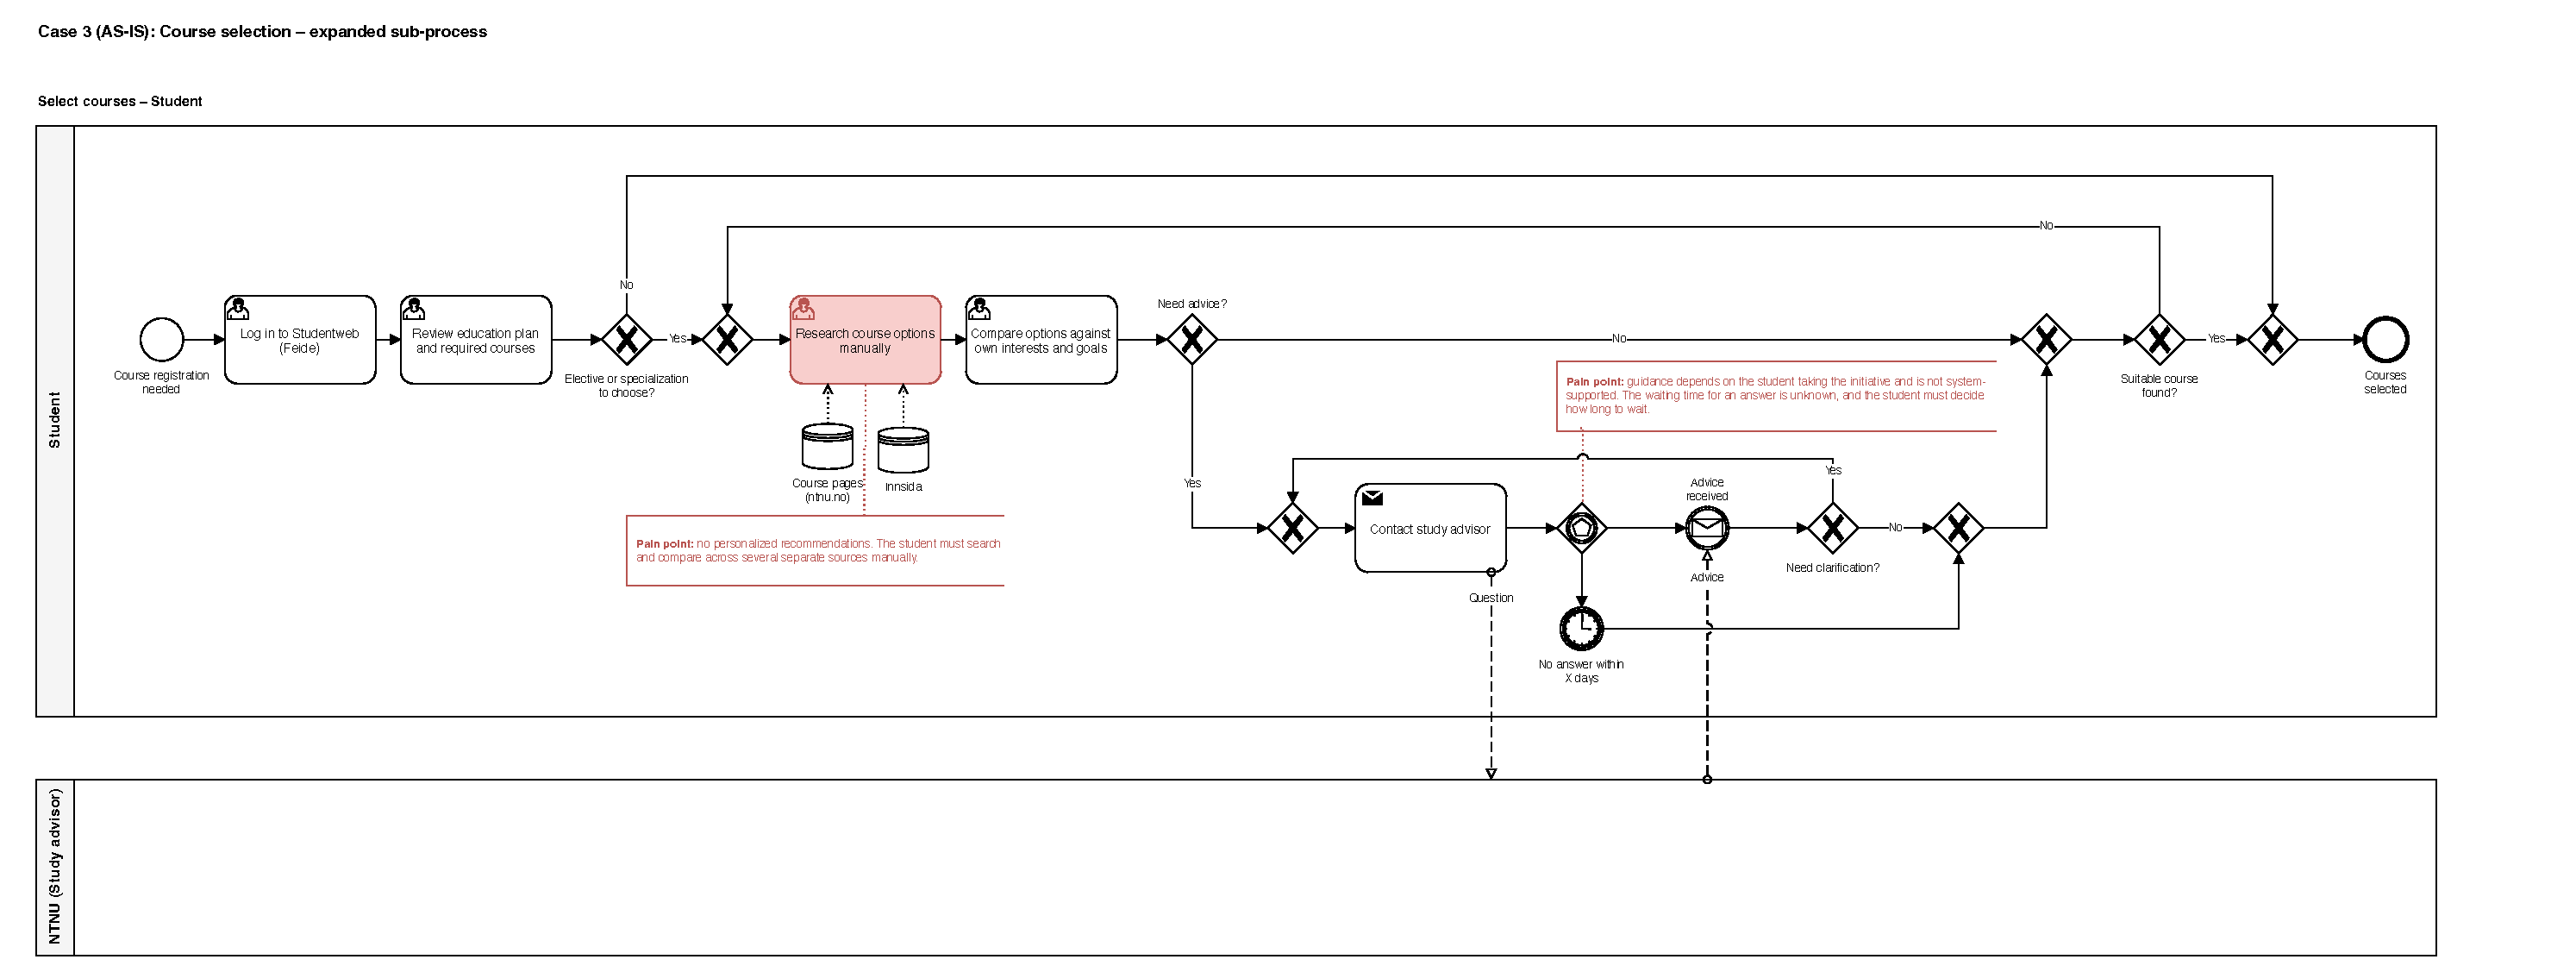
\includegraphics[width=\textwidth]{Images/case3/case3_as-is.drawio.pdf}
    \caption{Case 3 BPMN model}
    \label{fig:case3}
\end{figure}

Figure~\ref{fig:case3} expands the collapsed subprocess "Select courses" from the main model (Figure~\ref{fig:main_as-is}). The model consists of two pools: Student and NTNU. The Student pool contains the subprocess itself, while NTNU is shown as a black-box pool, since the student only communicates with the study advisor through messages. The advisor's own work is shown in the Study advisor lane of the main model. Identified pain points are marked as annotations in the model.

The process starts in the Student pool when course registration is needed. The student logs in to Studentweb using Feide and reviews their education plan and required courses. An exclusive gateway then represents whether the student has to choose elective courses. If not, the subprocess ends directly, and the student continues to registration in the main model (Figure~\ref{fig:main_as-is}). If elective courses must be chosen, the student researches course options manually, using the NTNU course pages and Innsida as information sources, and compares the options against their own interests and goals. As highlighted in the model, there is no personalized recommendation at this stage, and the student must search and compare across several separate sources on their own.

After comparing the options, the student decides whether they need advice. If so, the student contacts a study advisor by sending a question to NTNU. The advisor then gives guidance on the course options and sends the advice back, which is shown in the "Study advisor" lane of the main model (Figure~\ref{fig:main_as-is}). On the student side, an event-based gateway represents the two possible outcomes. Either the advice is received, or no answer has arrived within a given number of days. The length of this waiting period is subjective and depends on how long each student is able to wait. If the advice is received, the student decides whether further clarification is needed. If needed, the study advisor is contacted again. The model highlights that this guidance depends on the student taking the initiative, is not supported by any system, and involves an unknown waiting time before an answer is given.

When the student has either received sufficient advice, chosen not to wait any longer, or did not need advice in the first place, an exclusive gateway checks whether a suitable course has been found. If not, the student returns to researching course options manually. If suitable course is found the subprocess ends with "Courses selected", and the student continues to registration in Studentweb, which is shown in the main model (Figure~\ref{fig:main_as-is}).

The model shows that course selection is largely manual and driven by the student. In the overall process, system support is limited to validating and storing the registration in Studentweb and FS, as shown in the main model (Figure~\ref{fig:main_as-is}). The step where the student has to decide what to choose, and the only point where personal guidance is available, depends entirely on the student’s own research and on the study advisor’s availability.

